\newpage


% \section{Extension WooCommerce}
% Le plugin agira comme un pont entre la boutique e-commerce et notre API :
% \begin{itemize}
%     \item \textbf{Configuration :} Saisie de l'API Key par local.
%     \item \textbf{Checkout :} Calcul dynamique des frais de livraison en fonction de la distance.
%     \item \textbf{Webhooks :} Envoi automatique des données de commande (adresse, téléphone, dimensions) dès validation du paiement client.
% \end{itemize}



\section{Conception de l'Extension WooCommerce (Plugin Commerçant)}
\label{sec:extension_woocommerce}

L'extension WooCommerce agit comme un pont invisible entre la boutique du commerçant et notre infrastructure logistique. Son rôle est d'intercepter les nouvelles commandes éligibles à la livraison express et de les transmettre de manière sécurisée à notre API.

\subsection{Directives Techniques : La Stack du Plugin}

Le développement dans l'écosystème WordPress impose des standards stricts pour garantir la compatibilité avec des milliers de thèmes et d'autres plugins.

\begin{itemize}
    \item \textbf{Langage (Backend) :} \textbf{PHP 8.2+}. Le code devra suivre les standards de codage WordPress (PSR-12 adaptés). L'utilisation de l'orienté objet (OOP) est obligatoire pour encapsuler la logique et éviter les conflits de nommage dans l'espace global.
    \item \textbf{Communication API :} Utilisation exclusive de la \textbf{WP HTTP API} (\texttt{wp\_remote\_post}, \texttt{wp\_remote\_get}) plutôt que cURL en direct. Cela garantit une meilleure gestion des timeouts et des certificats SSL natifs à WordPress.
    \item \textbf{Interface (Frontend \& Admin) :} \textbf{JavaScript Vanilla} ou \textbf{React} (via \texttt{@wordpress/scripts}). L'interface d'administration (pour saisir la clé API et voir le statut des livraisons) utilisera les composants natifs de l'interface WordPress pour une intégration visuelle transparente.
\end{itemize}

\subsection{Diagramme de Séquence : Interception d'une Commande (Le Hook)}

Dans WooCommerce, le cycle de vie d'une commande est régi par des "Hooks" (actions et filtres). Le diagramme ci-dessous montre comment le plugin écoute l'événement de paiement réussi pour déclencher la demande de livraison vers notre API.

\begin{figure}[ht!]
    \centering
    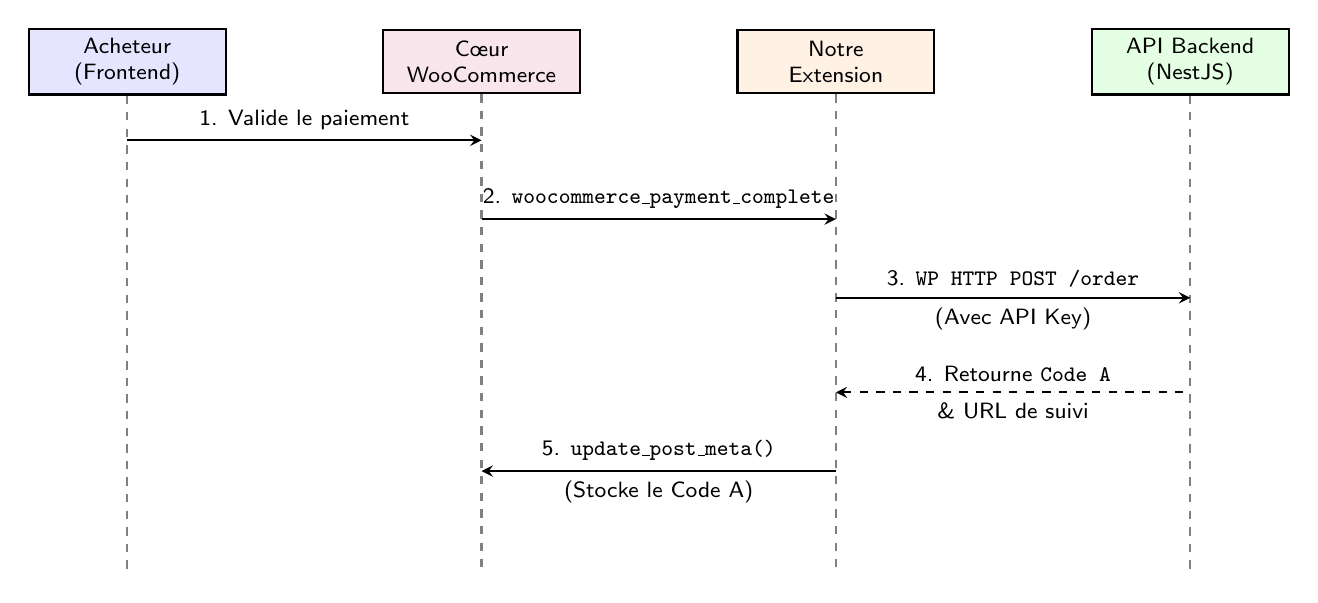
\begin{tikzpicture}[
        font=\sffamily\footnotesize,
        >=stealth,
        actor/.style={draw, thick, fill=gray!10, minimum width=2.5cm, minimum height=0.8cm, align=center},
        lifeline/.style={draw, dashed, thick, gray}
    ]

    % Entités
    \node[actor, fill=blue!10] (client) at (0, 0) {Acheteur\\(Frontend)};
    \node[actor, fill=purple!10] (woo) at (4.5, 0) {Cœur\\WooCommerce};
    \node[actor, fill=orange!10] (plugin) at (9, 0) {Notre\\Extension};
    \node[actor, fill=green!10] (api) at (13.5, 0) {API Backend\\(NestJS)};

    % Lignes de vie
    \draw[lifeline] (client) -- (0, -6.5);
    \draw[lifeline] (woo) -- (4.5, -6.5);
    \draw[lifeline] (plugin) -- (9, -6.5);
    \draw[lifeline] (api) -- (13.5, -6.5);

    % Séquence
    \draw[->, thick] (0, -1) -- node[above]{1. Valide le paiement} (4.5, -1);
    
    \draw[->, thick] (4.5, -2) -- node[above]{2. \texttt{woocommerce\_payment\_complete}} (9, -2);
    
    \draw[->, thick] (9, -3) -- node[above]{3. \texttt{WP HTTP POST /order}} node[below]{(Avec API Key)} (13.5, -3);
    
    \draw[<-, thick, dashed] (9, -4.2) -- node[above]{4. Retourne \texttt{Code A}} node[below]{\& URL de suivi} (13.5, -4.2);
    
    \draw[->, thick] (9, -5.2) -- node[above]{5. \texttt{update\_post\_meta()}} node[below]{(Stocke le Code A)} (4.5, -5.2);

    \end{tikzpicture}
    \caption{Séquence de création d'une course logistique via le plugin WooCommerce.}
    \label{fig:seq_woocommerce}
\end{figure}

\subsection{Directives Opérationnelles pour les Développeurs du Plugin}

Pour garantir que l'extension soit validée si elle est publiée sur le répertoire officiel WordPress, l'équipe devra respecter les points suivants :

\subsubsection{1. Sécurité et Stockage des Clés}
\begin{itemize}
    \item \textbf{Chiffrement :} La \texttt{Secret API Key} saisie par le commerçant dans les réglages ne doit pas être stockée en clair si possible, ou à minima restreinte aux administrateurs via la fonction \texttt{current\_user\_can('manage\_options')}.
\end{itemize}

\subsubsection{2. Résilience et Fallback (Tolérance aux pannes)}
\begin{itemize}
    \item \textbf{Gestion des pannes API :} Si notre API Backend est injoignable (Timeout), le plugin \underline{ne doit pas} bloquer le processus d'achat du client final. Il doit enregistrer la commande dans WooCommerce, l'ajouter à une file d'attente locale (Action Scheduler de WooCommerce), et réessayer la transmission (Retry Pattern) quelques minutes plus tard.
\end{itemize}

\subsubsection{3. Intégration à l'UI Commerçant (Back-office)}
\begin{itemize}
    \item \textbf{Méta-boîte (Meta Box) :} Les développeurs devront ajouter un encart spécifique sur la page de détail d'une commande (côté Admin WordPress). Cet encart affichera en gros le \textbf{Code A} (Handshake) à fournir au livreur, ainsi que le statut en temps réel de la course.
\end{itemize}